\chapter{Teoria sulla climatizzazione degli edifici}
\thispagestyle{empty}
L'essere umano ha il continuo desiderio di vivere un luogo in condizioni termo-igrometriche perfette. 

La teoria che si cela dietro l'attributo \emph{termo-igrometrico} è alla base della climatizzazione degli edifici.

Cosa si intende per \emph{climatizzazione}? Un edificio si definisce climatizzato o un impianto è di climatizzazione quando vengono controllati questi valori ambientali:
\begin{itemize}
	\item Temperatura;
	\item Umidità;
	\item Qualità dell'aria mediante un suo ricambio.
\end{itemize}
Il controllo di questi tre valori permette di vivere, come già è stato detto, un ambiente in condizioni termo-igrometriche ottimali. E solo un impianto di climatizzazione (solitamente un UTA -- \emph{Unità di Trattamento dell'Aria}) propriamente detto permette di ottenere questi risultati. Se, per esempio, non viene garantito il ricambio dell'aria (ovvero non viene immessa in ambiente una certa portata di aria esterna), l'impianto non è di climatizzazione. A tal proposito, i mono-split a compressione di vapore che abbiamo nelle nostre case non sono \emph{climatizzatori} ma dei semplici \emph{raffrescatori} (o \emph{riscaldatori} a seconda della stagione).

La domanda successiva a cui bisogna dare una risposta è la seguente: \emph{quali sono le condizioni termo-igrometriche ottimali?}

La risposta è complicata anche se alcuni progettisti termo-tecnici tenderebbero subito a rispondere: \n{25}{\degreeCelsius} col \n{40}{\%} in estate e \n{20}{\degreeCelsius} col \n{50}{\%} in inverno.

In verità, per rispondere concretamente a questa domanda bisogna introdurre la teoria sulla climatizzazione degli edifici. E per farlo si parte dal soggetto del primo periodo di questo capitolo: \emph{l'essere umano}.

\section{Il Comfort}
L'uomo, in quanto essere vivente, trasforma continuamente l'energia chimica presente negli alimenti in forme più consone al mantenimento in vita del proprio corpo e alla sua trasformazione: quest'attività prende il nome di \emph{metabolismo}.

Questa continua trasformazione produce calore che risulta variabile in base all'attività svolta: stare seduto, camminare, correre, fare attività pesante e così via.

Non è difficile concludere che, considerando l'essere umano come un sistema chiuso, questo calore prodotto produce un accrescimento della temperatura corporea. Idealmente fino all'infinito. Ovviamente, l'essere umano non è un sistema chiuso e questo calore interno deve essere smaltito in relazione alle condizioni climatiche dell'ambiente esterno e, contemporaneamente, deve garantire la temperatura interna corporea.

In termini matematici il tutto si traduce in questo bilancio di potenze
\begin{equation}
	\label{bilanciocorpoumano}
	S=M-W-E_d-E_{sw}-E_{ve}-C_{ve}-C-R-C_k
\end{equation}
dove:
\begin{description}
	\item[$\mathbf{S}$]Variazione di energia del corpo umano nell'unità di tempo o accumulo di energia termica nell'unità di tempo;
	\item[$\mathbf{M}$]Potenza metabolica;
	\item[$\mathbf{E_d}$] Potenza termica dispersa per diffusione attraverso la pelle;
	\item[$\mathbf{E_{sw}}$] Potenza termica dispersa per sudorazione attraverso la pelle;
	\item[$\mathbf{E_{ve}}$] Potenza termica dispersa nella respirazione come "calore latente";
	\item[$\mathbf{C_{ve}}$] Potenza termica dispersa nella respirazione come "calore sensibile";
	\item[$\mathbf{C}$] Potenza termica dispersa per convezione;
	\item[$\mathbf{R}$] Potenza termica dispersa per irraggiamento;
	\item[$\mathbf{C_k}$] Potenza dispersa per conduzione;
\end{description}
È risaputo che nel caso in cui la temperatura esterna sia eccessivamente alta o bassa, il meccanismo termoregolatorio del corpo tenda rispettivamente a far sudare il corpo stesso (smaltendo il calore tramite evaporazione del sudore) o a provocare i brividi (aumento dell'attività muscolare e quindi di calore prodotto). Nel caso in cui questi due ultimi meccanismi non siano sufficienti a mantenere costante l'energia interna del corpo si ha l'\emph{ipertermia} (fino alla morte per danni reversibili alle proteine dei tessuti nervosi) o l'\emph{ipotermia} (fino alla morte per fibrillazione cardiaca).

Quindi, è molto importante vivere in un ambiente che abbia delle condizioni termo-igrometriche tali da non provocare la morte prematura del proprio corpo.

Il vero problema è che queste così agognate \emph{condizioni termo-igrometriche ideali} non sono universali. E il motivo risiede nel fatto che ogni persona è diversa dalle altre. Infatti, ognuno tende a vestirsi diversamente (ovvero cambia la resistenza termica che il corpo oppone verso l'esterno e contemporaneamente anche il suo fattore di vista nel caso dell'irraggiamento) ma sopratutto ognuno tende ad avere un'attività metabolica $M$ completamente diversa. È come se ogni persona desiderasse una propria temperatura. Ovviamente è praticamente impossibile realizzare una cosa del genere in un ambiente affollato.

Citando da \emph{Impianti di climatizzazione per l'edilizia}~\cite{alfano}:
\begin{quote}
	Perché ci sia comfort termico, una condizione necessaria è che l'energia interna del corpo umano non aumenti nè diminuisca, ovvero che sia nullo il termine di accumulo che nella \ref{bilanciocorpoumano} è indicato come $S$; per $S=0$ questa equazione diventa una relazione del tipo:
	\begin{equation}
	\label{bilanciocorpoumanoSnullo}
		f(\mathrm{abbigliamento, attivit\grave{a}}, t_a, v_a, \Phi, t_r, t_{sk}, E_{sw})=0
	\end{equation}
	che lega tra loro otto variabili: due legate al soggetto (abbigliamento e attività), quattro ambientali (temperatura $t_a$, velocità $v_a$ e umidità~$\Phi$ dell'aria e temperatura media radiante $t_r$ -- ovvero temperatura di un ambiente fittizio termicamente uniforme che scambierebbe con l'uomo la stessa potenza termica radiante scambiata nell'ambiente reale) e due fisiologiche (temperatura della pelle $t_{sk}$ e potenza termica dispersa per sudorazione o percentuale di pelle bagnata dal sudore $E_{sw}$).
	
	In verità le due variabili fisiologiche non sono variabili indipendenti, ma dipendono con legge complessa dalle altre; 
	
	\sdots
	
	Secondo Fanger, perché siano verificate le condizioni di benessere, devono essere anche soddisfatte le due equazioni:
	\begin{gather}
	\label{Esw}
		E_{sw}=0.42A_b[(M-W)/A_b-58.2]\\
	\label{tsk}
		t_{sk}=35.7-0.0275(M-W)/A_b
	\end{gather}
	cioè i valori di $E_{sw}$ e di $t_{sk}$ reali in condizioni di comfort termico sono quelli che si ottengono dalle due ora scritte in funzione dell'attività realmente svolta dal soggetto.
	
	In definitiva le possibili condizioni di benessere termico sono le combinazioni delle sei variabili indipendenti che soddisfano contemporaneamente le equazioni \ref{bilanciocorpoumanoSnullo}, \ref{Esw} e la \ref{tsk}.
\end{quote}
Col tempo sono stati definiti degli indici che permettono di valutare il benessere termico in un locale. 

Uno di questi è il PMV (\emph{Predicted Mean Vote} -- Voto Medio Previsto): indipendentemente dal valore assunto dalle 6 variabili indipendenti, se 
\begin{equation}
\label{PMV}
	-0.5<\textrm{PMV}<0.5
\end{equation}
allora una condizione necessaria ma non sufficiente per il benessere è soddisfatta.

L'altra condizione che permette di vivere in un ambiente termicamente accettabile è l'assenza di \emph{discomfort localizzato}, causato da:
\begin{itemize}
	\item elevati gradienti verticali e orizzontali di temperatura;
	\item correnti d'aria.
\end{itemize}
Per tutte queste cause vi sono altrettanti indici che permettono di esprimere la presenza o meno di problematiche.

Quindi riassumendo: nel momento in cui le cause di discomfort localizzato sono assenti e il valore del PMV (che è un indice di discomfort \emph{globale} perché interessa tutto l'ambiente) è compreso nel suddetto intervallo (\ref{PMV}), allora l'ambiente stesso si può definire termo-igrometricamente accettabile. 

Per concludere questa parte sul comfort è bene precisare che, citando da \emph{Impianti di climatizzazione per l'edilizia}~\cite[pag 31]{alfano}
\begin{quote}
	gli indici esprimono la risposta media di un gran numero di soggetti, il che significa che per valori dell'indice corrispondenti per esempio a condizioni di comfort termico ci possono comunque essere individui che invece avvertono caldo o freddo.
\end{quote} 
È chiaro, quindi, che per ogni tipologia di locale (in cui verosimilmente le persone svolgono attività comuni) sono definiti dei valori che permettono di assicurare le condizioni di benessere. Solitamente, comunque, a meno di casi eccezionali in cui sono necessarie condizioni termiche altrettanto particolari, gli ambienti o i locali in cui le persone svolgono attività leggere, vestiti \emph{normalmente}\footnote{È in corsivo perché anche il vestiario è normato e quindi un capo di abbigliamento è diverso dall'altro e produce risultati diversi: non esiste un vestito \emph{normale}. Con questo termine mi riferisco, quindi, ad una tipologia di vestiario comune.} (quindi uffici e similari), in cui non si suda, i valori di temperatura e umidità sono quasi sempre quelli enunciati all'inizio di questo capitolo: \n{25}{\degreeCelsius} col \n{40}{\%} in estate e \n{20}{\degreeCelsius} col \n{50}{\%} in inverno.
\section{Il Carico Termico}
Dopo aver definito il comfort in un ambiente, è necessario calcolare il carico termico che consente di dimensionare l'impianto che permetta di realizzare quelle condizioni termo-igrometricamente accettabili di cui si è parlato nel paragrafo precedente.

\subsection{Carico Termico Invernale}
Con \emph{carico termico invernale} si definisce una potenza termica che l'edificio, in precisate condizioni univocamente definite, disperde verso l'ambiente esterno. Le suddette \emph{condizioni definite} sono:
\begin{itemize}
	\item il clima, ovvero i \emph{parametri climatici esterni} che costituiscono le sollecitazioni esterne sul sistema edificio. Questi parametri sono di disturbo perchè allontanano le condizioni termiche dell'ambiente interno da quelle desiderate di benessere. Queste cause sono:
	\begin{itemize}
		\item la differenza di temperatura tra l'aria interna e quella esterna;
		\item il vento che investe l'edificio;
		\item la radiazione solare incidente.
	\end{itemize}
	Per una valutazione approssimativa del carico termico invernale, è essenziale conoscere perlomeno la differenza di temperatura tra interno e esterno. La velocità dell'aria, invece, è importante se si vuole considerare anche lo scambio termico convettivo. L'apporto solare non viene considerato nel carico invernale in quanto è un beneficio perché tende a riscaldare l'ambiente interno e quindi, per questioni di sicurezza, viene ignorato;
	\item l'edificio, inteso come involucro edilizio che racchiude e delimita lo spazio interno nel quale si vogliono imporre le condizioni di benessere per gli occupanti, diventa così il confine fisico tra esterno ed interno e caratterizza fortemente l'interazione termica tra i due ambienti con le sue proprietà geometriche e termofisiche. Progettare un impianto di riscaldamento significa quindi mettere a punto un sistema capace di neutralizzare nell'ambiente interno gli effetti prodotti prevalentemente dal clima esterno;
	\item l'impianto è lo strumento con cui mantenere nell'ambiente riscaldato le condizioni volute contrastando le perturbazioni indotte dalle variazioni climatiche esterne.
\end{itemize}
La trattazione sui carichi termici invernali non si occupa degli aspetti igrometrici e di quant'altro attiene al vapor d'acqua, si affrontano cioè le sole problematiche legate al cosiddetto \emph{calore sensibile}, ossia agli scambi di calore che manifestano i loro effetti sulla sola temperatura di bulbo asciutto dell'aria esterna.

Da un'analisi energetica sull'edificio, si ricava la seguente relazione:
\begin{equation}
	\dot{Q}_{\textrm{risc}}=\dot{Q}_T+\dot{Q}_V-\dot{Q}_{\textrm{sor}}-\dot{Q}_{\textrm{sol}}
\end{equation}
Solitamente non potendo confidare con certezza in tutta la stagione negli apporti gratuiti interni $\dot{Q}_{\textrm{sor}}$ e solare $\dot{Q}_{\textrm{sol}}$ nell'equazione che definisce il carico termico invernale questi ultimi vengono trascurati. Per cui il \emph{carico termico invernale} è definito attraverso la seguente relazione:
\begin{equation}
\label{caricotermico:invernale}
\dot{Q}_{\textrm{risc}}=\dot{Q}_T+\dot{Q}_V+\dot{Q}_{\textrm{ripr}}
\end{equation}
dove $\dot{Q}_T$ è il carico termico invernale dovuto alla trasmissione tramite l'involucro dell'edificio e $\dot{Q}_V$ è quello dovuto al riscaldamento dell'aria immessa (con un impianto di ventilazione o tramite semplice infiltrazione naturale) all'interno dell'edificio stesso per portarlo alle condizioni desiderate di progetto. L'ultimo termine viene introdotto in quanto, secondo la \norinv\ sugli \emph{Impianti di riscaldamento negli edifici -- Metodo di calcolo del carico termico di progetto} serve a tener conto della potenza termica aggiuntiva, detta di \emph{ripresa}, necessaria a compensare gli effetti del regime intermittente dell'impianto di riscaldamento.

Il calcolo del carico termico invernale si fonda su tre ipotesi:
\begin{itemize}
	\item Trascurabilità degli apporti gratuiti: ovvero non si considera la $\dot{Q}_{\textrm{sor}}$ e la $\dot{Q}_{\textrm{sol}}$;
	\item Condizione statisticamente più sfavorevole: in questo modo l'impianto sarà sempre in grado di mantenere le condizioni di benessere all'interno dell'edificio;
	\item Regime stazionario: la principale grandezza climatica che ha la capacità di produrre un regime transitorio nell'edificio è la radiazione solare che si è detta trascurabile in inverno.
\end{itemize}

In base alla norma \norinv, la $t_e$ è la temperatura dell'aria esterna di progetto del luogo ove è ubicato l'edificio in esame ed è necessaria per il calcolo della $\dot{Q}_{\textrm{risc}}$. L'ipotesi di \emph{regime stazionario} obbliga a scegliere per il calcolo delle dispersioni una temperatura dell'aria esterna che sia costante (quando evidentemente non lo è perché si tratta di un parametro climatico) e che sia caratteristica delle condizioni meteorologiche del luogo e del clima in cui sorge l'edificio oggetto del calcolo. L'ipotesi delle \emph{condizioni più sfavorevoli} porterebbe a scegliere una temperatura che sia la più bassa tra quelle che stagionalmente si verificano nel corso degli anni nella località in cui l'edificio si trova. Solo in questo caso si sarebbe sicuri di calcolare un carico di picco per l'impianto sufficiente a garantire nell'ambiente riscaldato la temperatura $t_i$ anche al presentarsi delle sollecitazioni esterne più avverse.

Il problema con la seconda ipotesi risiede nel fatto che se si considera la temperatura più bassa degli ultimi, per esempio, 10 anni, si andrebbe a costruire un impianto molto sovradimensionato in quanto quella stessa temperatura potrebbe non aversi per alcuni anni e nel frattempo l'impianto non verrebbe sfruttato al 100\%. 

Proprio per queste ragioni l'ipotesi di \emph{condizioni più sfavorevoli} va in generale coniugata alle esigenze pratiche ed economiche. A tale scopo per stabilire la temperatura esterna di progetto sono stati sviluppati metodi alternativi al precedente. Un criterio già usato in Canada e negli Stati Uniti definisce la $t_e$ come la media delle temperature minime assolute del mese più freddo calcolata su un certo numero di anni. Questa è assunta pari alla temperatura a cui corrisponde un \emph{frequenza cumulata} pari al 97.5\% per gli edifici costruiti con materiali pesanti o normali e del 99\% per quelli di materiale leggero. Per \emph{frequenza cumulata} si intende la percentuale dei valori orari di temperatura che risultano superiori ad un determinato limite. Ad esempio, dire che la frequenza cumulata del valore $t_e=-5$\ \si{\degreeCelsius} è del 97.5\%, significa che nell'arco di un determinato intervallo temporale, scelto come rappresentativo del periodo più freddo per quella località, c'è solo il 2.5\% di probabilità che si verifichi per la $t_e$ un valore più basso. Con ciò si ammette implicitamente che nel 2.5\% dei giorni di quel periodo possano verificarsi delle condizioni climatiche tali da non permettere all'impianto di garantire la temperatura interna $t_i$ nella zona riscaldata perchè il valore delle dispersioni termiche supera il carico di picco che l'impianto è in grado di bilanciare.

\subsection{Carico Termico Estivo}
Il calcolo dei carichi termici estivi, rispetto al caso invernale, è più complesso a causa della dinamicità dei fenomeni. In particolare, mentre per il calcolo delle dispersioni invernali si fa riferimento a condizioni stazionarie, nel caso delle rientrate estive ciò non è possibile a causa dell'estrema variabilità nelle ore del giorno dei flussi termici legati alla radiazione solare. Questi ultimi, di lieve entità nella stagione invernale (e pertanto trascurati in quanto sono anche apporti gratuiti in conflitto con le ipotesi di calcolo del carico termico invernale), costituiscono ora un carico termico assolutamente non trascurabile a cui l'impianto deve fare fronte.

L'irradiazione solare è un carico \emph{rotante} in quanto è variabile durante la giornata. Quando l'involucro dell'edificio viene "colpito" dalla radiazione solare, questo tende a riscaldarsi esternamente molto più di quanto non lo faccia la temperatura esterna. Questa potenza termica aggiuntiva, quindi, entrando all'interno dell'involucro riscalda l'ambiente interno per convezione e irraggiamento. Bisogna definire due fenomeni molto importanti che prendono il nome di \emph{sfasamento} e \emph{attenuazione} che fanno capo all'\emph{inerzia termica} della struttura. A causa di questi due fenomeni il carico termico che giunge all'interno risulta essere in ritardo (sfasamento) e di minore intensità (attenuazione) rispetto alla radiazione che colpisce esternamente l'involucro. Siccome è importantissimo bilanciare questi carichi l'ideale sarebbe quelli di attenuarli e sfasarli quanto è più possibile: in questo modo il carico esterno risulta essere costante durante tutte le 24h. 

A differenza della trattazione sui carichi termici invernali ci si occupa in questo caso anche degli \emph{aspetti igrometrici} e di quant'altro attiene al vapore d'acqua; si affrontano dunque sia le problematiche legate al calore sensibile che a quello latente. Al controllo della temperatura si aggiunge spesso in regime estivo quello dell'umidità. Alla semplicità della valutazione dei carichi termici invernali si contrappone quella più complessa nel caso estivo. E lo si può tranquillamente notare di seguito dove vengono classificati i carichi termici estivi.
\begin{description}
	\item[Carichi Termici Sensibili] $ $
	\begin{itemize}
		\item radiazione solare attraverso i vetri;
		\item trasmissione attraverso vetri, muri e tetti;
		\item infiltrazione di aria esterna;
		\item carico interno all'ambiente dovuto a persone, luci, apparecchiature elettriche;
	\end{itemize}
	\item[Carichi Termici Latenti] $ $
	\begin{itemize}
		\item apporto di vapore dovuto a persone presenti in ambiente;
		\item infiltrazione di aria esterna, avente in genere un'umidità specifica superiore a quella dell'aria ambiente;
		\item vapore prodotto in ambiente da eventuali processi o apparecchiature presenti.
	\end{itemize}
\end{description}
Il tutto si riassume nella seguente relazione di calcolo del \emph{carico termico estivo}:
\begin{equation}
	\label{caricotermico:estivo}
	\dot{Q}_{\textrm{frigo}}=\dot{Q}_{\textrm{sol}}+\dot{Q}_T+\dot{Q}_{\textrm{sor}}+\dot{Q}_V
\end{equation}
Siccome il carico $\dot{Q}_{\textrm{sol}}$ risulta essere rotante, il calcolo di $\dot{Q}_{\textrm{frigo}}$ dovrà effettuarsi ora per ora nell'arco della giornata. La potenzialità dell'impianto di climatizzazione è quindi determinata in base al massimo carico corrispondente ad una data ora della giornata. Nelle restanti ore la potenza frigorifera richiesta all'impianto sarà sempre inferiore a quella disponibile. D'altro canto conviene non sovradimensionare troppo il gruppo frigorifero poichè se questo funziona troppo lontano dalla sua potenzialità nominale sarà caratterizzato da basse efficienze energetiche o troppo frequenti intermittenze operative. 

\subsection{L'edificio}
Dopo aver valutato i carichi termici nelle due stagioni si vuole sottolineare l'importanza delle proprietà termo-fisiche dell'involucro dell'edificio.
La base della teoria sulla trasmissione del calore si basa su questa semplice equazione:
\begin{equation}
	\dot{Q}=UA\mathit{\Delta} T
\end{equation}
Ovviamente la $\dot{Q}$ viene causata dal $\mathit{\Delta} T$ per mezzo della trasmittanza $U$: siccome si è detto che si cerca di avere la $\dot{Q}$ quanto più bassa possibile, bisogna intervenire certamente e in modo più diretto sulla resistenza offerta dall'involucro dell'edificio: impossibile certamente agire sul $\mathit{\Delta} T$. La superficie, invece, può essere progettata in modo tale che il carico termico sia più equilibrato sfruttando l'orientamento, le correnti d'aria prevalenti e, nel caso, anche ombre naturali (o costruendone di artificiali).

È necessario a questo punto introdurre gli elementi costruttivi di un edificio poco energivoro.

\subsubsection{Stagione Invernale}
Le ipotesi di \emph{regime stazionario} semplificano di molto la stima del carico termico. Anche la scelta dei materiali dell'involucro non è impegnativa. Si cerca, infatti, di avere una trasmittanza tale da contenere la potenza termica entrante. Si agisce essenzialmente sulla $U$. Al giorno d'oggi il Decreto Ministeriale del~26~Giugno~2015 chiede di contenere questi valori di trasmittanza entro quelli riportati nella tabella \vref{vallim:opve} valida per le strutture opache verticali soggette a riqualificazione.
\begin{table}
	\centering
	\begin{tabular}{ccc}
		\multirow{2}{*}{Zona Climatica} & \multicolumn{2}{c}{\textbf{U} [\trasm]}	\\
		\cmidrule(lr){2-3}
										& \textbf{2015} & \textbf{2021}				\\
		\midrule
		A e B							&	0.45		&	0.40 					\\
		C								& 	0.40		&	0.36					\\
		D								&	0.36		&	0.32					\\
		E								&	0.30		&	0.28					\\
		F								&	0.28		&	0.26					\\
	\end{tabular}
	\caption{Valori limite per la trasmittanza\\strutture opache verticali -- DM 26/6/2015}\label{vallim:opve}
\end{table}
Tabelle simili sono presenti nello stesso decreto per le superfici opache orizzontali, oblique e per i componenti trasparenti.

Bisogna spendere qualche parola sui componenti trasparenti. Questi, infatti, rappresentano le superfici più delicate all'interno di un edificio. Innanzitutto introducono una discontinuità materiale e geometrica all'interno di una parete: questo comporta un'alterazione del campo termico che in una parete è assimilabile ad un campo piano (cioè la parete si può tranquillamente studiare come una lastra piana). Dove sono presenti gli infissi, il campo termico viene alterato diventando bidimensionale e intensificando la potenza termica trasmessa. Il secondo aspetto che li rende delicati è il fatto che sono trasparenti: se ciò risulta essere un beneficio in inverno, non lo è assolutamente in estate. È necessario, quindi, sfruttare la radiazione solare in inverno per risparmiare sul riscaldamento mentre bisogna evitarla in estate.

Per fare ciò si sono studiati dei trattamenti superficiali a cui sottoporre i vetri. Quelli dedicati alla stagione invernale rendono il vetro quanto più trasparente possibile alla radiazione solare (sopratutto sulle lunghezza d'onda del visibile) ma opachi sull'infrarosso.

I vetri a \emph{guadagno solare} hanno un'elevato comportamento trasmissivo sulle frequenze del visibile mentre quelli \emph{bassoemissivi} sono opachi su quelle dell'infrarosso. Quest'ultima tipologia di trattamento evita la fuoriuscita dall'edificio (tramite gli infissi ovviamente) della radiazione emessa dai corpi presenti all'interno dell'edificio: corpi che in inverno risultano essere certamente più caldi dell'esterno.
\newpage
\subsubsection{Stagione Estiva}
Come è già stato ampiamente detto lungo tutto questo capitolo, alla \emph{stazionarietà} della stagione invernale si contrappone la \emph{dinamicità} della stagione estiva provocata dalla radiazione solare.

Essa, infatti, rappresenta un carico termico non indifferente e di cui bisogna tenere debitamente conto. Anzi, al giorno d'oggi e alle nostre latitudini meridionali, è quasi più importante progettare l'involucro di un edificio per "resistere" alla stagione estiva che non a quella invernale. Facendo un semplice ragionamento, infatti, è possibile capire come proprio la radiazione solare rappresenti un punto cruciale per la progettazione, appunto, dell'involucro stesso.

Considerando un edificio sito a Napoli, dalla \norvent\ si hanno questi valori di temperatura esterna:
\begin{itemize}
	\item \n{2}{\degreeCelsius} per la stagione invernale;
	\item \n{32}{\degreeCelsius} per la stagione estiva;
\end{itemize}
All'interno dell'edificio, invece, non si devono superare i \n{20}{\degreeCelsius} nella stagione invernale mentre in estate un buon livello di benessere si ottiene con \n{25}{\degreeCelsius}.

È facile notare che, a parità di involucro (e quindi di trasmittanza termica), il salto termico è maggiore in inverno (\n{18}{\degreeCelsius}) che in estate (\n{7}{\degreeCelsius}). Da ciò potremmo concludere che l'involucro debba essere di tipo resistivo (bassa trasmittanza) per resistere, appunto, al forte gradiente termico che si instaura in inverno. 

La realtà delle cose è ben diversa. Questo modo di procedere va molto bene nei Paesi del Nord Europa dove gli inverni sono molto rigidi (si scende tranquillamente sotto gli \n{0}{\degreeCelsius}) mentre le temperature estive sono confortevoli.

Alle nostre latitudini (\ang{41}), invece, l'estate è rappresentata da temperature molto più elevate ma sopratutto da una radiazione solare incidente notevole: si raggiungono i \n{300}{W/m^2}. Il tutto si traduce in un aumento di temperatura delle superfici esposte al sole. Questo fenomeno non è per niente trascurabile. Infatti, nella valutazione del carico termico estivo si usa solitamente la \emph{temperatura sole-aria} ($t^{'}_e$): nell'ipotesi che il solo scambio esterno fosse per convezione, la suddetta temperatura è quella che genera la stessa potenza termica che nella realtà viene scambiata anche per irraggiamento.

Per rendere l'idea di quanto l'irraggiamento giochi un ruolo cruciale in estate, questa $t^{'}_e$ è pari a \n{61.6}{\degreeCelsius} il 21 Luglio (16:00) alle latitudini napoletane su una superficie esposta a Ovest quando alla stessa ora la temperatura esterna è circa \n{34.4}{\degreeCelsius}. 

Nel caso estivo non bisogna usare la stessa metodologia invernale: ovvero limitare la trasmittanza per diminuire il carico proveniente dall'esterno. Infatti, come è stato detto nel paragrafo precedente, la stagione estiva, essendo molto dinamica, introduce all'interno dell'edificio onde termiche molto consistenti: si cerca di realizzare l'involucro in modo tale che queste onde siano più attenuate e sfasate possibili.

I muri da utilizzare devono essere molto \emph{capacitivi}: questo lo si realizza con materiali che possiedono o un'elevata capacità termica o realizzando involucri che siano molto massivi. In questo modo la funzione congiunta della capacità termica e della trasmittanza provoca onde sfasate e attenuate. Il risultato ideale è quello di carico termico costante e limitato tutta la giornata. Questo modo \emph{innovativo} di progettare gli involucri nella stagione estiva è consigliato anche nel Decreto Ministeriale del 26 Giugno 2015 dove si legge:
\begin{quote}
	Ad esclusione della zona F per le località in cui il valore medio mensile dell'irradianza sul piano orizzontale nel mese di massima insolazione $I_{m,s} \ge \SI{290}{W/m^2}$, verificare che:
	\begin{itemize}
		\item per le pareti opache verticali (ad eccezione di quelle nel quadrante Nord-Ovest/Nord/Nord-Est) sia rispettata almeno una delle seguenti condizioni:
		\begin{itemize}
			\item $M_s > \SI{260}{kg/m^2}$
			\item $Y_{IE}<\SI{0.10}{W/m^2K}$
		\end{itemize}
		\item per tutte le pareti opache orizzontali e inclinate, che:
		\begin{itemize}
			\item $Y_{IE}<\SI{0.18}{W/m^2K}$
		\end{itemize}
	\end{itemize}
	dove:\\
	$M_s$: rappresenta la massa superficiale della parete opaca compresa la malta dei giunti ed esclusi gli intonaci [\si{kg/m^2}];\\
	$Y_{IE}$: rappresenta la trasmittanza termica periodica valutata in accordo con UNI EN ISO 13786:2008 e successivi aggiornamenti [\si{W/m^2K}].
	
	Note:
	\begin{itemize}
		\item Gli effetti positivi che si ottengono con il rispetto dei valori di massa superficiale o trasmittanza termica periodica delle pareti opache, possono essere raggiunti, in alternativa, con l'utilizzo di tecniche e materiali, anche innovativi, ovvero coperture a verde, che permettano di contenere le oscillazioni della temperatura degli ambienti in funzione dell'irraggiamento solare. \sdots
		
	\end{itemize}
\end{quote}

Il problema vero e proprio nasce con i componenti trasparenti che permettono, per loro natura, alla radiazione solare di entrare all'interno degli edifici.

I vetri a \emph{controllo solare} sono stati sviluppati per proteggere l'ambiente interno dalla radiazione solare stessa. Essi comprendono:
\begin{itemize}
	\item I vetri \emph{selettivi} hanno un un elevato valore di $\tau$ in corrispondenza delle onde visibili della radiazione solare per poi annullarsi in corrispondenza del vicino infrarosso. Siccome la banda a cui i vetri sono trasparenti è molto stretta (proprio per evitare ingressi indesiderati), la $\tau$ è lievemente bassa anche nel visibile e pertanto il vetro risulta essere leggermente più scuro;
	\item i vetri \emph{assorbenti} hanno un elevato valore  di $\alpha$ nel visibile: ciò si traduce con un vetro apparentemente scuro. La problematica di questo trattamento risiede nel fatto che assorbendo la radiazione solare, il vetro tende a riscaldarsi in poco tempo e quindi trasmettere verso l'interno un'aliquota della radiazione solare incidente sulle onde dell'infrarosso: immaginando una parete vetrata di questa tipologia, in poco tempo è come avere una parete radiante che annulla totalmente i benefici di un trattamento per il \emph{controllo solare} estivo. Quindi, un vetro di questo genere viene sempre accoppiato con uno basso-emissivo in modo tale che la radiazione emessa dalla lastra assorbente viene bloccata da quella basso-emissiva. Ovviamente una configurazione di questo genere viene montata in modo tale che il vetro a controllo solare sia posto esternamente.
	\item i vetri \emph{riflettenti} hanno un elevato valore della riflessività su tutta la banda a partire dal visibile: ad occhio nudo appaiono come specchi.
\end{itemize}

Da tutto ciò discendono queste conclusioni (o modi di progettare l'edificio):
\begin{itemize}
	\item In inverno è molto importante avere una trasmittanza bassa per limitare lo scambio termico con l'esterno (sia per i componenti opachi che trasparenti). I componenti trasparenti, inoltre, per migliorare il guadagno solare (ovvero permettere alla radiazione solare di entrare negli edifici diminuendo il carico termico da abbattere con gli impianti) dovrebbero venir posizionati in maniera rilevante sopratutto sulle superfici esposte a sud;
	\item In estate i componenti opachi dovrebbero avere una elevata \emph{trasmittanza termica periodica} in modo tale che l'onda di calore dovuta alla radiazione solare incidente la parete venga attenuata e sfasata opportunamente. I componenti trasparenti dovrebbero essere limitati, se non addirittura assenti, sulle superfici esposte a est e ovest. A sud il problema dell'ingresso di radiazione solare tramite il vetro a guadagno solare viene risolto posizionando esternamente tendine o coperture: il sole in estate risulta, come è ben noto, più alto sulla volta celeste mentre è più basso in inverno. 
	\item A nord il componente trasparente non deve essere presente o, al limite, lo si sceglie del tipo \emph{basso-emissivo} per contenere le dispersioni di radiazione infrarossa.
	\item Bisogna sfruttare quanto è più possibile le correnti d'aria prevalenti in una determinata zona così da favorire il \emph{free cooling} estivo durante la notte. 
	\item È doveroso effettuare un'analisi accurata degli ombreggiamenti durante tutto l'anno per abbattere (o quantomeno diminuire) il carico termico che l'impianto deve bilanciare.
\end{itemize}
\section{I Software}
L'analisi dei carichi e dei fabbisogni energetici è stata effettuata con l'ausilio di software basati sulla tecnologia \bim.

Il \bim\ (\emph{Building Information Modelling}) è un metodo che, citando da \textit{Wikipedia.it}, permette:
\begin{quote}
	\dots l'ottimizzazione della pianificazione, realizzazione e gestione di costruzioni tramite aiuto di un software. Tramite esso tutti i dati rilevanti di una costruzione possono essere raccolti, combinati e collegati digitalmente. La costruzione virtuale è visualizzabile inoltre come un modello geometrico tridimensionale.%\footnote{https://it.wikipedia.org/wiki/Building\_Information\_Modeling}
\end{quote}
Si sta lavorando a livello Europeo affinché questa metodologia di progettazione possa avere una sua definizione. Al giorno d'oggi, infatti, il BIM viene frainteso con una qualche sorta di tecnologia o addirittura software: niente di più sbagliato. Gli applicativi basati sulla \emph{filosofia del BIM} hanno delle peculiarità che li differenziano in modo marcato dagli altri. Infatti in un programma BIM un oggetto (per esempio un edificio) viene rappresentato tridimensionalmente perché disegnato da un architetto ma ogni parte di questo edificio contiene delle informazioni utili ad uno strutturista (ovvero tipologia del materiale usato per un muro o anche le sue caratteristiche fisiche). Continuando in questa direzione, altre informazioni che è possibile inserire in questo edificio (o file) sono le caratteristiche termiche dell'involucro (opaco e trasparente), il disegno/progettazione dei vari impianti (idraulici, aeraulici e elettrici). Una volta inserite tutte queste informazioni è possibile ricavare dei dati molto preziosi. Per esempio il carico termico nella stagione estiva/invernale, il computo metrico del materiale utilizzato, fare stime e/o studi sulla vita utile dell'edificio, etc\dots

Tutte queste informazioni sono presenti all'interno di un unico file. E siccome il file è unico, viene incentivata la cooperazione tra i diversi professionisti. Addirittura è possibile lavorare contemporaneamente su quest'unico file in modo tale che una modifica di una parte del progetto si ripercuote automaticamente sugli altri aspetti progettuali cosicché le altre figure professionali vengono automaticamente avvertite di suddetta modifica. Questo si traduce in una maggiore velocità di esecuzione, una sostanziale diminuzione di errori e costi di progettazione.

Citando dal sito della software-house ACCA:
\begin{quote}
	Grazie alla metodologia del BIM l'edificio viene "costruito" prima della sua realizzazione fisica, mediante un modello virtuale, attraverso la collaborazione ed i contributi di tutti gli attori coinvolti nel progetto (architetti, ingegneri, progettisti, consulenti, analisti energetici, etc\dots).
\end{quote}
Nello studio di riqualificazione energetica in questione, il programma utilizzato è costituito da una suite di applicativi diversi che si interfacciano in modo tale da realizzare ciò che la metodologia BIM impone.

Di \textbf{CYPE}, ovvero la suite, sono stati usati i seguenti programmi:
\begin{description}
	\item[IFC Builder]permette di disegnare geometricamente l'edificio definendo di volta in volta i suoi elementi (involucro opaco e trasparente, locali e zone termiche). Il file \textsc{.ifc} realizzato permette di essere esportato e utilizzato da qualsiasi altro programma che supporta questo file. Il formato \textsc{.ifc} è aperto, libero e ben documentato. In parole povere: questo file è alla base del BIM in quanto permette la cooperazione tra diversi programmi (usati rispettivamente da diverse figure professionali);
	\item[CYPETHERM Loads]permette di definire le caratteristiche termo-fisiche dell'involucro e la destinazione d'uso dei locali importati dal file \textsc{.ifc}. Restituisce i carichi termici (annuali, mensili e orari) per ogni locale delle zone termiche. Una volta ottenuti i risultati è possibile esportarli in modo tale che qualsiasi altro programma della suite CYPE possa utilizzarli;
	\item[CYPETHERM HVAC]permette di importare i file realizzati con IFC Builder e Loads e progettare/dimensionare un adeguato impianto HVAC per l'abbattimento del carico sensibile e latente oltre che per il rinnovo dell'aria;
	\item[CYPETHERM C.E.]permette di effettuare la certificazione energetica degli edifici rispettando la normativa UNI TS-11300.
\end{description}
In \vref{bim:cype} è riassunto il funzionamento della suite di CYPE. Si noti la centralità del server \emph{BIMserver.center} a cui tutti i progetti prodotti dai vari programmi fanno capo.
\begin{figure}[h]
	\centering
	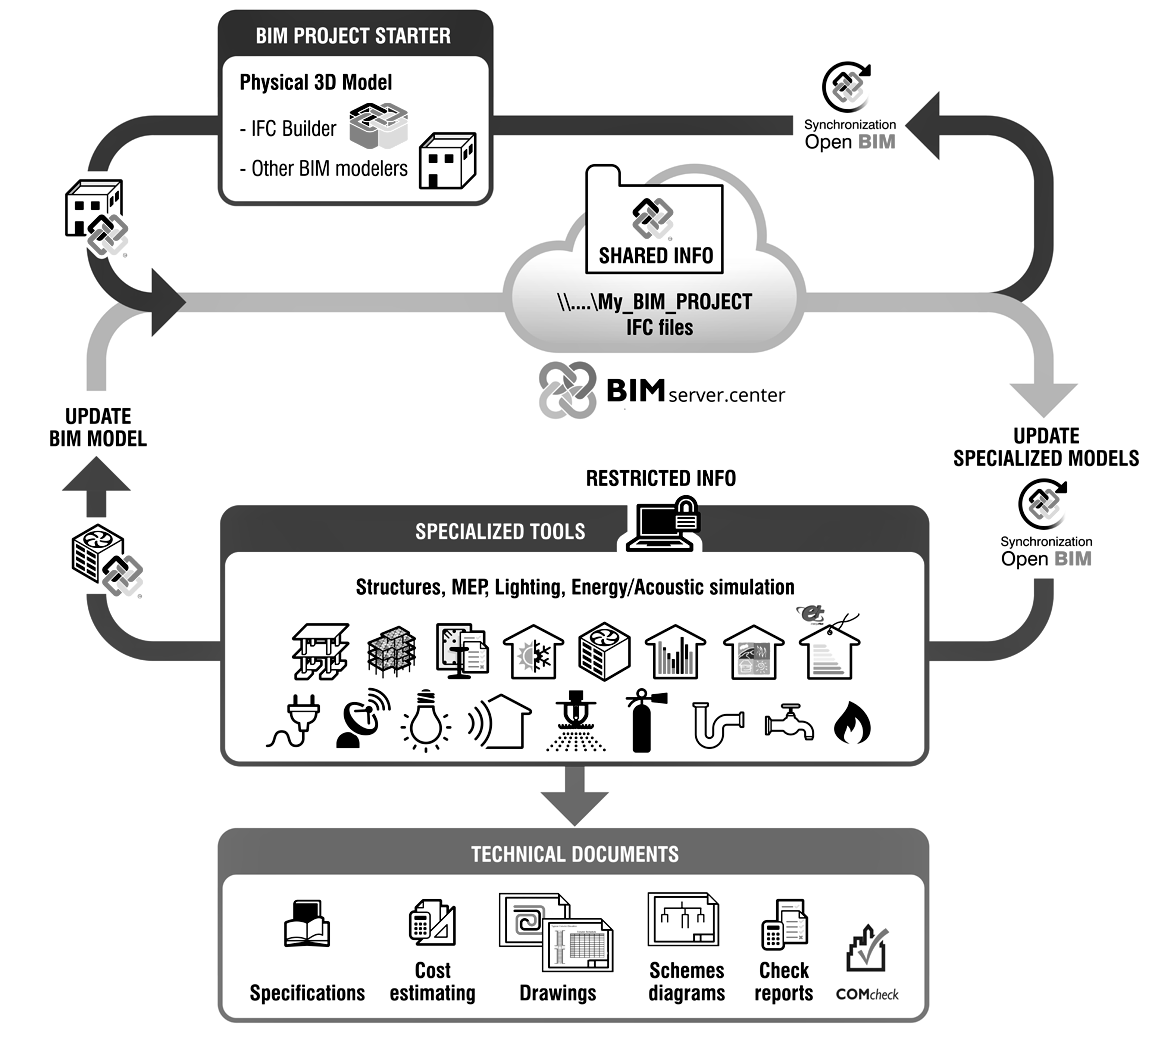
\includegraphics[width=0.5\textheight]{6_2_cap/img/cypeflow}
	\caption[Schema della filosofia BIM per CYPE]{Schema riassuntivo del funzionamento\\ della \emph{suite} CYPE con filosofia BIM.}
	\label{bim:cype}
\end{figure}

Per quanto riguarda la parte idronica si è utilizzato un applicativo BIM della software-house \emph{C.A.T.S.} che si appoggia ad \emph{Autodesk Autocad}.

È stato possibile definire inizialmente la tipologia di tubazioni da utilizzare (dimensioni, materiale e coibente), la metodologia di dimensionamento con le velocità minime ammissibili e poi disegnare direttamente in Autocad le tubazioni stesse posizionando le unità locali (radiatori e fancoil). Infine, l'applicativo ha dimensionato le tubazioni, rilasciato il computo metrico e la relazione di calcolo.